\section{Evaluacija}
\label{sec:ImplementationExample}

U ovom odeljku će biti prikazano nekoliko slučajeva upotrebe implementirane aplikacije. Prvo će biti pokazan primer generisanja opšteg AST u JSON formatu a zatim i primer poređenje dve implementacije istog algoritma u dva različita programska jezika. Algoritam koji će biti korišćen u nastavku kao primer je algoritam razmene vrednosti promenljivih implementiran kroz funkciju \texttt{swap} koja menja vrednosti dveju globalnih promenljivih. Na slici \ref{fig:ExampleSwap} se mogu videti implementacije ovog algoritma koje će biti polazne tačke za kreiranje opšteg AST i poređenja istih.

\begin{figure}[h!]
\begin{lstlisting}
int x = vx, y = vy;
void swap() { int tmp = y; y = x; x = tmp; }
\end{lstlisting}
\begin{lstlisting}
x = vx
y = vy
function swap()
	x, y = y, x
end
\end{lstlisting}
\begin{lstlisting}
algorithm Swap 
begin
    declare integer x = vx
    declare integer y = vy
    procedure swap()
    begin
        declare integer tmp 
        tmp = x
        x = y  
        y = tmp
    end
end
\end{lstlisting}
\caption{Izvorni kodovi algoritma \texttt{swap} u programskim jezicima C (gore), Lua (sredina) i u pseudojeziku (dole).}
\label{fig:ExampleSwap}
\end{figure}


\subsection{Generisanje opšteg AST}
\label{subsec:ImplementationExampleAST}

AST je moguće generisati od izvornog koda navođenjem glagola \texttt{ast}. Ukoliko su dostupni izvorni kodovi sa sadržajima kao na slici \ref{fig:ExampleSwap} u odgovarajućim datotekama, moguće je generisati opšti AST u JSON formatu zadavanjem glagola \texttt{ast} kao na slici \ref{fig:ExampleSwapAST}. U gornjem delu slike je prikazan samo deo izlaza zbog veličine generisanog JSON sadržaja, u srednjem delu slike je prikazan kompaktni JSON ispis zadat opcijom \texttt{-c}, dok je u donjem delu slike prikazan ispis zadat opcijom \texttt{-v} pri čemu je prikazan samo dao izlaza koji se generiše prilikom posećivanja stabla parsiranja i generisanja AST čvorova.

\begin{figure}[h!]
\centering
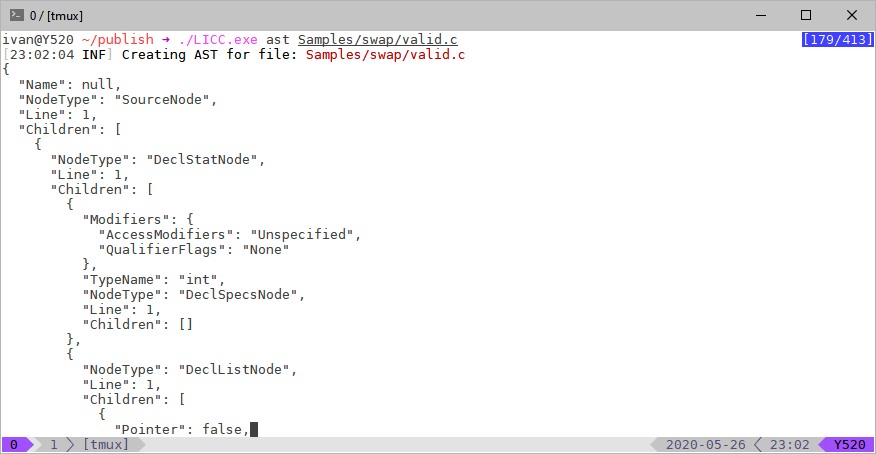
\includegraphics[scale=0.56]{images/eval/ast_c.png}
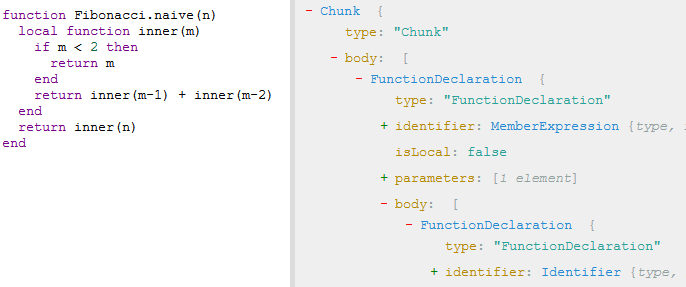
\includegraphics[scale=0.56]{images/eval/ast_lua.png}
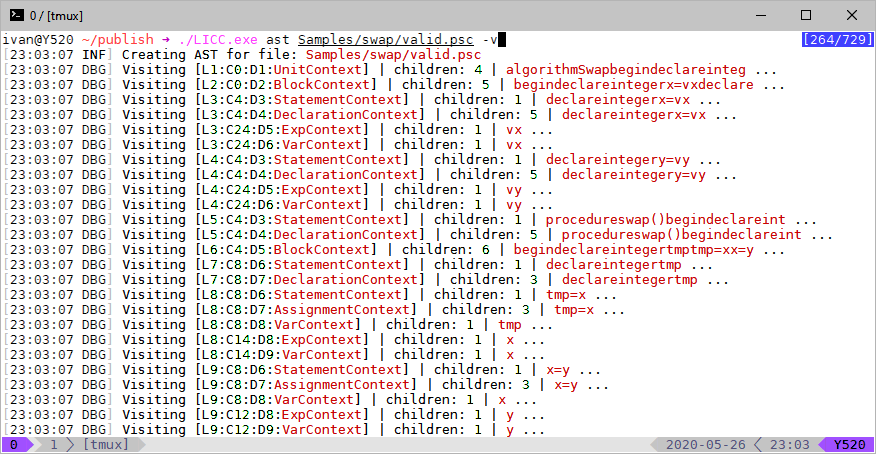
\includegraphics[scale=0.56]{images/eval/ast_psc.png}
\caption{Vizualni prikaz generisanja AST od izvornih kodova sa slike \ref{fig:ExampleSwap} redom.}
\label{fig:ExampleSwapAST}
\end{figure}

U okviru repozitorijuma projekta je moguće pronaći još primera upotrebe. Na stranici \url{https://github.com/ivan-ristovic/LICC/LICC.AST/Samples} se mogu naći izvorne datoteke u kojima su iskorišćene sve podržane sintaksičke strukture od kojih se može kreirati AST. Izvorne datoteke su pisane u programskim jezicima C, Lua i pseudojeziku (po jedna za svaki programski jezik). Ove datoteke u okviru projekta služe kao integracioni testovi ali čitaocu mogu dati jasan uvid u koncepte koje LICC podržava u zavisnosti od programskog jezika. U okviru repozitorijuma se nalaze i uputstva za kreiranje novih graditelja i upoređivača.


\subsection{Poređenje opštih AST}
\label{subsec:ImplementationExampleComparer}

Jedan od osnovnih slučajeva upotrebe alata LICC može biti testiranje validnosti implementacije na osnovu date specifikacije, koja ne mora biti pisana u istom programskom jeziku kao i implementacija. Ukoliko kao specifikaciju za algoritam \texttt{swap} uzmemo izvorni kod u pseudo-jeziku, možemo testirati da li su implementacije u programskim jezicima C ili Lua semantički ekvivalentne specifikaciji. Izlaz rada LICC za verifikaciju implementacije algoritma \texttt{swap} u programskom jeziku Lua u odnosu na specifikaciju u pseudo-jeziku se može videti na slici \ref{fig:ExampleSwapCompareValid}. Primetimo da su prisutna upozorenja o odudaranju tipova promenljivih i funkcija --- Lua nije striktno tipiziran jezik, a specifikacija nalaže da su globalne promenljive celi brojevi, dok su u implementaciji one tipa \texttt{object}, dok funkcija \texttt{swap} može imati i povratnu vrednost. S obzirom na prirodu skript jezika ovakve razlike nisu prijavljene kao greške, već samo kao upozorenja. 

\begin{figure}[h!]
\centering
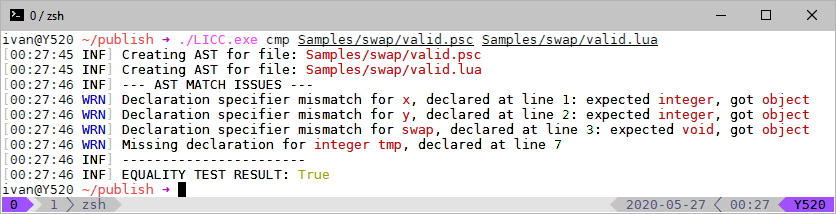
\includegraphics[scale=0.65]{images/eval/cmp_valid.png}
\caption{Semantičko poređenje implementacija sa slike \ref{fig:ExampleSwap} (Lua u odnosu na pseudo-jezik).}
\label{fig:ExampleSwapCompareValid}
\end{figure}

Ukoliko pak izvorni k\^od ne odgovara specifikaciji, LICC će dati detaljan spisak razlika, koje su često tražene greške. U nekim slučajevima je moguće da je sematnička ekvivalentnost održana iako stabla imaju značajne razlike --- LICC će prijaviti sve te razlike kao greške iako one to možda nisu. Izlaz za poređenje nevalidne implementacije algoritma \texttt{swap} sa slike \ref{fig:ExampleSwapWrong} u odnosu na specifikaciju se može videti na slici \ref{fig:ExampleSwapCompareWrong}. Vidimo da jedna od globalnih promenljivih nije pravilno zamenila vrednost, što se detektuje dvaput --- po jednom za svaki od blokova u izvornom kodu. Dodatno, prijavljena je i greška o odudaranju izraza inicijalizatora za promenljivu \texttt{tmp}.

\begin{figure}[h!]
\begin{lstlisting}
int x = vx, y = vy;
void swap() { int tmp = x; y = tmp; x = y; }
\end{lstlisting}
\caption{Nevalidna implementacija algoritma \texttt{swap} (C).}
\label{fig:ExampleSwapWrong}
\end{figure}

\begin{figure}[h!]
\centering
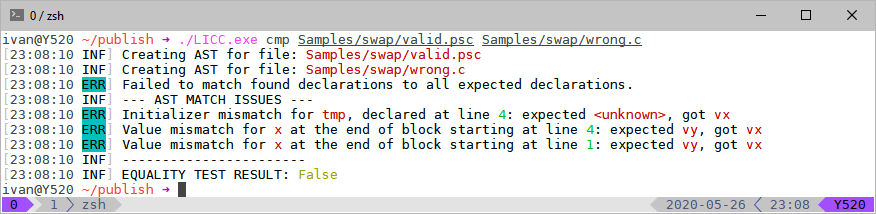
\includegraphics[scale=0.65]{images/eval/cmp_wrong.png}
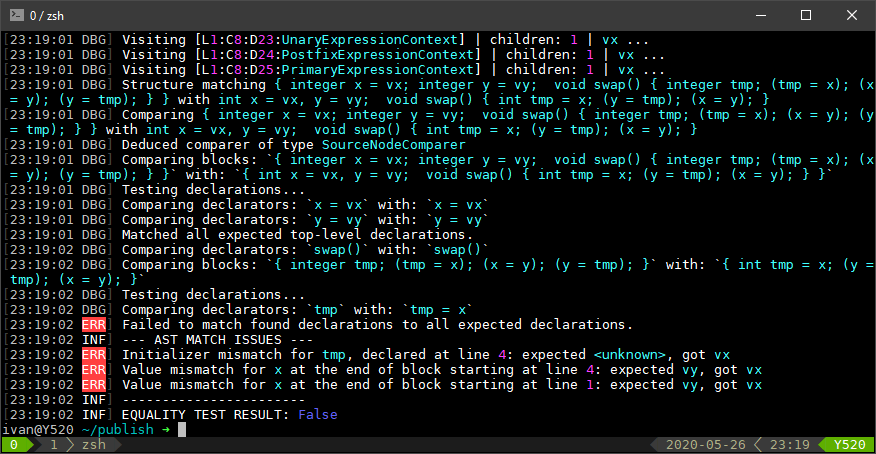
\includegraphics[scale=0.65]{images/eval/cmp_wrong_v.png}
\caption{Semantičko poređenje nevalidne implementacije sa slike \ref{fig:ExampleSwapWrong} u odnosu na specifikacije sa slike \ref{fig:ExampleSwap} -- C (gore) i pseudojezik (dole).}
\label{fig:ExampleSwapCompareWrong}
\end{figure}

Ukoliko imamo već verifikovanu implementaciju algoritma u jednom programskom jeziku, može se desiti potreba za prelaskom na novije tehnologije što uključuje i prepisivanje algoritma sa jednog programskog jezika na drugi. LICC se može iskoristiti za poređenje tih implementacija, konkretno za algoritam \texttt{swap} na slici \ref{fig:ExampleSwapCompareValidRewrite} se može videti rezultat poređenja implementacija u programskim jezicima C i Lua, pri čemu je takođe prikazan izlaz koji se dobija ukoliko se navede opcija \texttt{-v}. 

\begin{figure}[h!]
\centering
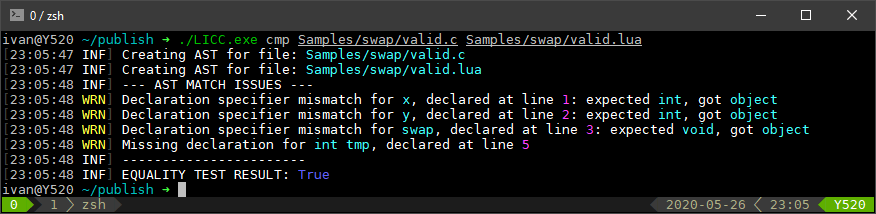
\includegraphics[scale=0.7]{images/eval/cmp_rewrite.png}
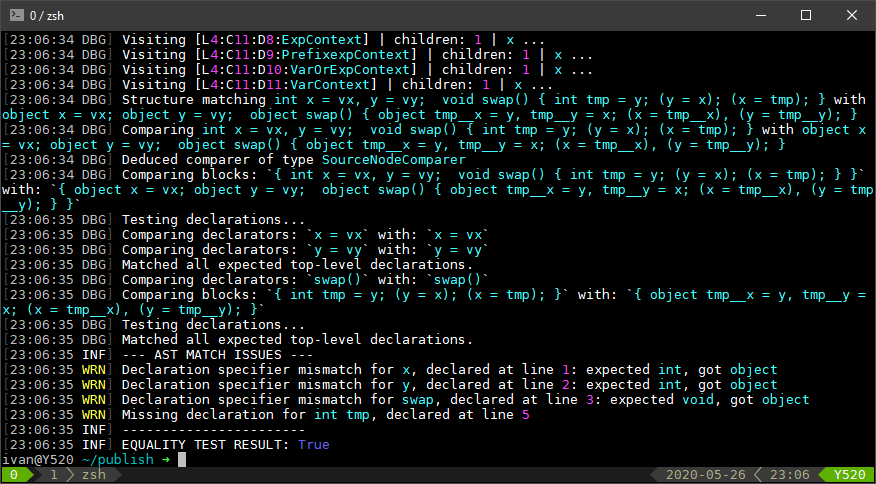
\includegraphics[scale=0.7]{images/eval/cmp_rewrite_v.png}
\caption{Semantičko poređenje implementacija sa slike \ref{fig:ExampleSwap} --- Lua u odnosu na C (gore), Lua u odnosu na pseudojezik (dole, sa detaljnim ispisom).}
\label{fig:ExampleSwapCompareValidRewrite}
\end{figure}

Još jedan slučaj upotrebe LICC može biti verifikacija međuverzija koda u procesu refaktorisanja. LICC pretpostavlja strukturnu sličnost kodova, što u procesu refaktorisanja često implicitno važi, ili barem važi u malim koracima između polazne i finalne verzije nakon refaktorisanja. 
%Ukoliko refaktorišemo implementaciju algoritma \texttt{swap} u programskom jeziku C i dobijemo izvorni kod sa slike \ref{fig:ExampleSwapRefactor}, možemo uporediti tu implementaciju sa već verifikovanom implementacijom u programskom jeziku C. Rezultat rada upoređivača se može videti na slici \ref{fig:ExampleSwapCompareRefactor} --- primećujemo da je jedino detektovano da nedostaje promenljiva \texttt{tmp}, vrednosti globalnih promenljivih su iste u odnosu na specifikaciju na kraju svakog od blokova.

% \begin{figure}[h!]
% \begin{lstlisting}
% int x = vx, y = vy;
% void swap() { x = x + y; y = x - y; x = x - y; }
% \end{lstlisting}
% \caption{Refaktorisani algoritam \texttt{swap} (C).}
% \label{fig:ExampleSwapRefactor}
% \end{figure}

% \begin{figure}[h!]
% \centering
% 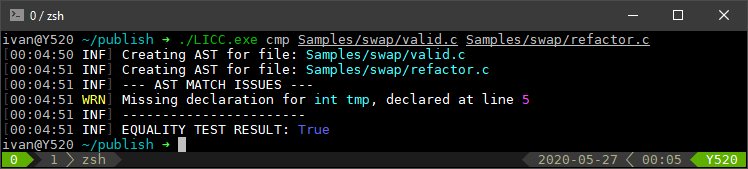
\includegraphics[scale=0.75]{images/eval/cmp_refactor.png}
% \caption{Semantičko poređenje refaktorisane implementacije algoritma \texttt{swap} sa slike \ref{fig:ExampleSwapRefactor} sa implementacijom u programskom jeziku C sa slike \ref{fig:ExampleSwap}.}
% \label{fig:ExampleSwapCompareRefactor}
% \end{figure}

Kompletan prikaz rada alata LICC za algoritam razmene vrednosti se može naći u okviru repozitorijuma na adresi \url{https://github.com/ivan-ristovic/LICC/LICC.Core/Samples/swap}. U okviru ovog direktorijuma su, uz ispravne i izmenjene izvorne datoteke algoritma, pružene i slike izlaza alata LICC za svaki par izvornih datoteka.

Kao primer prikaza poređenja deklaratora (promenljivih, nizovnih i funkcijskih), dat je primer koji se može pogledati na stranici \url{https://github.com/ivan-ristovic/LICC/LICC.Core/Samples/declarations}. Ovaj primer ilustruje poređenje više naredbi deklaracija čiji redosled nije nužno isti u izvornim datotekama, kao i detektovanje razlika u deklaratorima. U okviru ovog primera takođe se pokazuje i evaluacija izraza, kroz inicijalizatore celobrojnih i nizovnih promenljivih. Pošto je reč o deklaracijama, pružene su samo izvorne datoteke u programskom jeziku C i to validni primer, primer sa greškom kao i refaktorisani primer uz rezultate međusobnog poređenja parova izvornih datoteka.

Kao primer prikaza poređenja definicija funkcija sa parametrima, dat je primer koji se može pogledati na stranici \url{https://github.com/ivan-ristovic/LICC/LICC.Core/Samples/fparams}. Ovaj primer ilustruje poređenje funkcija čiji parametri utiču na rezultate analize unutar definicije funkcije. Kao primer prikaza poređenja kompleksnih naredbi, dat je primer koji se može pogledati na stranici \url{https://github.com/ivan-ristovic/LICC/LICC.Core/Samples/conditions}. Ovaj primer ilustruje poređenje naredbi grananja, pri čemu se detektuju izmene u uslovima grananja ali i odvojenim granama. Izvorne datoteke u okviru ova dva primera su pisane u programskim jezicima C, Lua i pseudojeziku i sastoje se od validnog primera, primera sa greškom i refaktorisanog primera uz rezultate međusobnog poređenja parova izvornih datoteka. Treba napomenuti da je provera bazirana na uparivanju grana uslova a zatim njihovom poređenju, što znači da se naredbe grananja koje imaju zamenjene grane i negiran uslov neće biti detektovane kao ekvivalentne.
